\documentclass[12pt]{article}

% Math and symbol packages
\usepackage{amsmath}
\usepackage{amssymb}
\usepackage{derivative}

% Figure Packages
\usepackage{graphicx}
\usepackage{wrapfig}
\usepackage{epstopdf}
\usepackage{float}
\usepackage{subfigure}
\usepackage{afterpage}

% Formatting and Random Text Generation
\usepackage{inputenc}
\usepackage[left=2.54cm,right=2.54cm,top=2.54cm,bottom=2.54cm]{geometry}
\usepackage{lipsum}

% Header and indent packages
\usepackage{fancyhdr}
\usepackage{indentfirst}

% Create Title Section
\title{Simple Harmonic Motion \\ \small (SHM)}
\author{Trevor Swan \\
Department of Physics, Case Western Reserve University \\
Cleveland, OH 44016-7079}
\date{}

% Actual Lab content
\begin{document}
\pagestyle{fancy}
\fancyhf{}

% Load the title
\maketitle
\thispagestyle{fancy}
\renewcommand{\headrulewidth}{0pt}

% Set up Footers
\fancyfoot[L]{Trevor Swan}
\fancyfoot[C]{\thepage}
\fancyfoot[R]{Simple Harmonic Motion}

% Abstract section of Report
\section{Abstract}
I have tested the spring constant, torsion constant, and torsion modulus for two independent simple harmonic motion apparatuses by using principles of linear and rotational harmonic motion. Using Newton's Second Law, I recorded an angular frequency $\omega$ for an apparatus with a spring to be $\omega=7.673\pm0.003\ s^{-1}$. Using this value, I calculated a spring constant of $k_s=2.94\pm0.06\ \frac{N}{m}$. I then used a similar expression based off similar principles to determine the angular frequency for the same apparatus with added weight. The calculated value of $\omega_p=5.72\pm0.07 s^{-1}$ does not align with the experimentally determined value as a result of minor systematic errors in the spring. Since the spring is not always properly taken care of, the expected spring constant is not going to necessarily align with the experiment itself, impacted the value of $\omega_p$. I then determined a value for the torsion constant of a translational pendulum using the angular analogue of Newton's Second Law to be $k_t=2.14\pm0.05\ N\cdot m$. Using this value, I calculated the torsion modulus for the rod in the apparatus to be $n=5.46\times10^{10}\pm0.52\times10^{10} \frac{N}{m^2}$. This value does not align with the given moduli for possible materials for the rod, so I concluded that the rod must be some Copper-Iron alloy.The discrepancy here is most likely due to misuse of the apparatus over time combined with improper measurement techniques in the lab. Systematic errors plagued the calculations and experiments done in this lab, preventing sound and confident conclusions.

% Introduction and Thoery
\section{Introduction and Theory}
Translational, or linear, harmonic motion can be analyzed and calculated using springs and Newtons Second Law. When a spring with given spring constant $k_{s}$ experiences a shift $x$ from its equilibrium position $x_0$, it exerts a restoring force according to:

% Restoring force
\begin{equation}
    F = -k_s(x-x_0) \label{restoring force}
\end{equation}

\noindent According to Newton's Second Law $F=ma$, we can rewrite Equation \ref{restoring force} as:

% N2L relation
\begin{equation}
    a = \frac{F}{m}=\frac{-k_s(x-x_0)}{m} \label{N2L restoring}
\end{equation}

\noindent We can then set up a Second Order Differential Equation using the fact that $a=\frac{d^2x}{dt^2}$:

% DE for Translational
\begin{equation}
    -k_s(x-x_0) = m\frac{d^2x}{dt^2} \label{DE trans}
\end{equation}

\noindent Using the principles of Differential Equations, we can then derive the general solution:

% General Solution
\begin{equation}
    x=x_m\sin(\omega t+\phi)+x_0 \label{trans general sol}
\end{equation}

\noindent where

% Omega expression trans
\begin{equation}
    \omega=\sqrt{\frac{k_s}{m}} \quad\text{and}\quad k_s = \omega^2m\label{Omega trans}
\end{equation}

For the above relationships, $x_m$ is given as the oscillation amplitude, $x_0$ is the spring's equilibrium position,  $\phi$ is the phase angle where the wave crosses its equilibrium with a positive slope for the first time, and $\omega$ is the angular frequency which can be expressed as seen in Equation \ref{Omega trans} or as:

% Representation of omega 
\begin{equation}
     \omega=2\pi f=\frac{2\pi}{T} \label{omega freq}
\end{equation}

By analogue, angular, or rotational harmonic motion can be analyzed using an elastic rod with a torsion constant $k_t$ . When twisted at an angle $\theta$, the restoring torque is:

% Restoring torque
\begin{equation}
    \tau = -k_t\theta \label{restoring torque}
\end{equation}

\noindent According to the rotational analogue of Newton's Second Law $\tau=I\alpha$, we can rewrite Equation \ref{restoring torque} as:

% NSL Rot relation
\begin{equation}
    -k_t\theta=I\alpha
\end{equation}

\noindent We can set up a Second Order Differential Equation similar to that in Equation \ref{DE trans}:

% DE for angular
\begin{equation}
    -k_t\theta=I\frac{d^2\theta}{dt^2} \label{DE angular}
\end{equation}

\noindent Using the principles of Differential Equations, we can then derive the general solution:

% General Solution
\begin{equation}
    \theta = \theta_m\sin(\omega t+\phi) \label{angular general sol}
\end{equation}

The above relationships contain nearly identical contents when compared to Equation \ref{trans general sol}, though $\omega$ can be determined through the following expression:

% Omega expression angular
\begin{equation}
    \omega=\sqrt{\frac{k_t}{I}} \label{Omega Rot}
\end{equation}

The fact that our apparatus uses a solid cylindrical plate allows us to derive the expression for $I$:

% Inertia of cyl
\begin{equation}
    I=\frac{1}{2}MR^2 \label{inertia cyl}
\end{equation}

We can then combine Equations \ref{omega freq}, \ref{Omega Rot}, and \ref{inertia cyl} to derive an expression for $k_t$ as follows:

% k_t expression with intertia params
\begin{equation}
    \begin{split}
        \omega^2=\frac{k_t}{I}\quad\therefore\quad k_t=I\omega^2=&\frac{1}{2}MR^2(\frac{2\pi}{T})^2=\frac{M(\frac{D}{2})^2}{2}\cdot\frac{4\pi^2}{T^2} \\ \\
        \rightarrow k_t=& \frac{\pi^2MD^2}{2T^2} \label{kt derivation}
    \end{split}
\end{equation}

We can also present the torsion constant $k_t$ as an expression in terms of the rod's parameters. For the expression below, $A$ is the cross-sectional area, $n$ is the torsion modulus of the material, and $L$ is the length of the rod. The expression is as follows:

% k_t expression with rod param
\begin{equation}
    k_t=\frac{nA^2}{2\pi L} \label{kt expression}
\end{equation}

Since the rod is a cylinder, it has circular cross sections that have an area that can be presented as $A=\pi(\frac{D}{2})^2$, where $D$ is the rod's diameter. Using this expression and Equation \ref{kt expression}, we can solve for the torsion modulus $n$ as follows:

% torsion modulus expression
\begin{equation}
    n=\frac{2\pi L k_t}{A^2}=\frac{2\pi L k_t}{(\pi(\frac{D}{2})^2)^2}=\frac{2\pi L k_t}{\pi^2\frac{D^4}{16}}=\frac{32 L k_t}{\pi D^4}\label{torsion modulus}
\end{equation}
It should also be noted that creating a histogram of the distribution of the periods of the pendulum should roughly follow a Gaussian distribution if the calculations and experiments are performed properly. \par
Finally, we can safely assume that the moment of inertia in the rod is negligible when compared to the cylinder because of the noticeable differences between the bodies masses and radii.

% Procedure
\section{Experimental Procedure}

% Explaining Spring with Mass
\subsection{Translational SHM}
We started our experiment with the Apparatus seen in Figure 1a. We first measured the weight our hanging mass to be $0.050\pm0.001\ kg$. We decided on this uncertainty as it aligns with the precision of our labs scale. We then attached the hanging mass to a ring stand positioned directly above a sonic motion detector, which would send position information to \textit{Logger Pro}. Before running any experiments, we ensured that our detector was functioning properly by running \textit{Logger Pro} with a lab notebook moving over the detector. \par

% Insert the Image of the apparatus
\begin{wrapfigure}{R}{0.5\textwidth}
  \begin{center}
    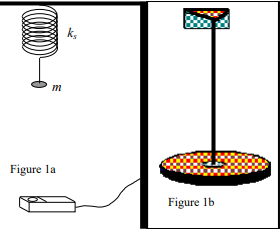
\includegraphics[width=0.48\textwidth]{SHM_Setup.png}
  \end{center}
  \caption{Experimental Apparatuses}
  \label{apparatus}
\end{wrapfigure}

To conduct the experiment itself, we lowered the spring a distance of about $4cm$ from its equilibrium position and released it when \textit{Logger Pro} was ready to collect data. We used \textit{Logger Pro's} fitting software to record the values of the sinusoidal oscillations seen in Equation \ref{trans general sol}. We repeated this 3 more times to ensure that our data was consistent and could be used to calculate uncertainties. Then, we conducted a similar experiment, altering the distance we pulled the spring from its equilibrium to about $10\ cm$. Finally, we returned to the $4\ cm$ position, but added a measured mass of $0.040\pm 0.001\ kg$ to the hanger to conduct this test. For both of these alterations, we recorded the constants \textit{Logger Pro} provided us. Again, the derivation of our chosen uncertainty is from the precision of our lab's scale ($\frac{1}{10}\ g$). \par

% Explaining torsional pendulum.
\subsection{Rotational SHM}
The second experiment we conducted made use of the apparatus seen in Figure 1b. We started by measuring the length of the rod and diameters of the plate and rod. To measure the length of the rod, we measured from its connection to the plate to the rod's connection to the table. This resulted in a measurement of $0.8571\pm0.0001\ m$. We decided on this uncertainty because the graduations on our meter stick went to the nearest millimeter, so we could estimate one decimal place after that. To measure the rod's diameter, we used \textit{Vernier} Calipers. We measured a diameter of $0.0043\pm0.0001\ m$. Our reasoning for the uncertainty in this measurement is similar to that of the rod's length, as the calipers are only so precise. Finally, we measured a plate diameter of $0.2555\pm 0.0005\ m$. Determining an accurate measurement of the diameter of the plate proved to be difficult because of the rods placement, so we accounted for this by increasing the uncertainty from the assumed $0.0001\ m$ produced by our meter sticks. We were also given the mass plate as we were unable to remove it in lab. Our plate was the Gray Iron plate, which had a mass of $4.6\pm0.1\ kg$. \par


To conduct the experiment itself, we twisted the plate just under $40^\circ$ to prevent damage to the apparatus. Using \textit{Logger Pro}, we recorded about 25 oscillations after releasing the plate in such a way that allowed a vertical rod to pass through a Photogate senor. We repeated this experiment until we had data that appeared to oscillate around a fixed value.

% Results and Analysis
\section{Results and Analysis}

% Needed analysis for hanging mass apparatus
\subsection{Translational SHM}
First, we determined an accurate measurement of the angular frequency $\omega$ but finding the average value, $\Bar{\omega}$, of our 4 trials using the second column in Table \ref{Sonic Motion Trials}:

% Caluclation for a good omega
\begin{equation*}
    \Bar{\omega}=\frac{7.672+7.681+7.670+7.670}{4}=7.673
\end{equation*}

\noindent Although $\Bar{\omega}=7.673\ s^{-1}$ is the correct notation for this quantity, I will refer to it simplify as $\omega$.

Then, we determined the estimated uncertainty for a single measurement $\sigma$, by using the below formula and technology to handle the calculation itself as it is too long and redundant to include in this report.

% STD expression
\begin{equation}
    \sigma=\sqrt{\frac{\sum^N_{i=1} (x_i - \Bar{x})^2}{N-1}} \label{STD Def}
\end{equation}

\noindent In this expression, $N$ is the number of samples in the dataset, in this case 4, and $x_i$ is the indexed value of the data in the set. For our data, we calculated $\sigma=0.0052599$.

Finally, we determined the error in the mean according to the following equation. $N$ represents the same quantity that is the number of values in the data set.

% Standard Error
\begin{equation}
    \delta = \frac{\sigma}{\sqrt{N}}
\end{equation}

\noindent For our data, we calculated $\delta_\omega=0.00263$.

Using this data we can propose a value for $\omega$ with its uncertainty which is $w = 7.673\pm0.003\ s^{-1}$. Further analyzing Table \ref{Sonic Motion Trials}, we compared this value with the measured $\omega$ value for the trial with increased amplitude. We observed that the large amplitude value of $\omega=7.672\pm0.001\ s^{-1}$ lies within the uncertainty of our calculated value above, showing that angular frequency is independent of amplitude.

We can then use Equation \ref{Omega trans} with this measured value for $\omega$ as well as a hanging mass weight $m=0.050\ kg$ to determine a value for the spring constant $k_s$:

% Spring constant Calculation
\begin{equation*}
    k_s= (7.673\ s^{-1})^2(0.050\ kg) = 2.944 \frac{N}{m}
\end{equation*}

\noindent We can also use Equation \ref{Omega trans} to determine the uncertainty in $k_s$ using the expression below:

% Uncertainty in k_s
\begin{equation}
    \delta_{k_s}=\sqrt{\delta_{k_s,\omega}^2+\delta_{k_s,m}^2} \label{UNC in ks}
\end{equation}

We can derive expressions for $\delta_{k_s,\omega}$ and $\delta_{k_s,m}$ using the derivative method and Equation \ref{Omega trans} as follows:

% Derivative calculations
\begin{align}
    % k due to omega
    \begin{split}
        \delta_{k_s,\omega}=\frac{\partial k_s}{\partial\omega}*\delta_\omega&=\frac{\partial}{\partial\omega}(\omega^2 m)*\delta_\omega \\
        &=2\omega m*\delta_\omega \label{ks due to omega}
    \end{split} \\ \nonumber \\
    % k due to m
    \begin{split}
        \delta_{k_s,m}=\frac{\partial k_s}{\partial m}*\delta_\omega&=\frac{\partial}{\partial m}(\omega^2 m)*\delta_m \\
        &=\omega^2*\delta_m \label{ks due to m}
    \end{split}
\end{align}

We can then compute the values of these uncertainties based on the values stated above. Here, we will use our measured values used to calculate $k_s$, and uncertainties $\delta_\omega=0.003\ s^{-1}$ and $\delta_m=0.001\ kg$. Substituting these values into Equations \ref{ks due to omega} and \ref{ks due to m} yields:

%Individual uncertainty calculations
\begin{align*}
    % k due to omega
    \begin{split}
        \delta_{k_s,\omega}=2(7.673)(0.050)*0.003=0.0023019
    \end{split} \\ \\
    %k due to m
    \begin{split}
        \delta_{k_s,m}=(7.673)^2*(0.001)=0.05887
    \end{split}
\end{align*}

We can then plug these values into Equation \ref{UNC in ks} to yield the following value of $\delta_{k_s}$:

% Calculation for delta k_s
\begin{equation*}
    \delta_{k_s}=\sqrt{0.0023019^2+0.05887^2}=0.0589\ \frac{N}{m}
\end{equation*}

\noindent With these two values, we can rewrite $k_s$ with its uncertainties as $k_s=2.94\pm0.06\ \frac{N}{m}$. \par

We can then use this value in conjunction with Equation \ref{Omega trans} to determine a theoretical value for $\omega_p$, the angular frequency of oscillations with an increased mass. Since we added a total of $0.040\ kg$ to the hanger, we can represent the mass as $m=0.090\pm0.001\ kg$. We can use this equation to make the following predictive calculation:

% wp calculation
\begin{equation*}
    \omega_p=\sqrt{\frac{2.944}{0.090}}=5.719\ s^{-1}
\end{equation*}

\noindent We can also use Equation \ref{Omega trans} to determine the uncertainty in $\omega_p$ using the expression below:

% UNC in omega p
\begin{equation}
    \delta_{\omega_p}=\sqrt{\delta_{\omega_p,k_s}^2+\delta_{\omega_p,m}^2} \label{UNC in omega p}
\end{equation}

We can derive expressions for $\delta_{\omega_p,k_s}$ and $\delta_{\omega_p,m}$ using the derivative method and Equation \ref{Omega trans} as follows:

% Derivative calculations
\begin{align}
    % omega due to k
    \begin{split}
        \delta_{\omega_p,k_s}=\frac{\partial\omega_p}{\partial k_s}*\delta_{k_s}&=\frac{\partial}{\partial k_s}(\sqrt{\frac{k_s}{m}})*\delta_{k_s} \\
        &=\frac{\sqrt{\frac{k_s}{m}}}{2k_s}*\delta_{k_s}\label{omega p due to k}
    \end{split} \\ \nonumber \\
    % omega due to m
    \begin{split}
        \delta_{\omega_p,m}=\frac{\partial\omega_p}{\partial m}*\delta_m&=\frac{\partial}{\partial m}(\sqrt{\frac{k_s}{m}})*\delta_{m} \\
        &=-\frac{\sqrt{\frac{k_s}{m}}}{2m}*\delta_m\label{omega p due to m}
    \end{split}
\end{align}

We can then compute the values of these uncertainties based on the values stated above. Here, we will use our measured values used to calculate $\omega_p$, and uncertainties $\delta_{k_s}=0.06\ \frac{N}{m}$ and $\delta_m=0.001\ kg$. Substituting these values into Equations \ref{omega p due to k} and \ref{omega p due to m} yields:

%Individual uncertainty calculations
\begin{align*}
    % omega due to k
    \begin{split}
        \delta_{\omega_p,k_s}=\frac{\sqrt{\frac{2.944}{0.090}}}{2(2.944)}*0.06=0.05828
    \end{split} \\ \\
    % omega due to m
    \begin{split}
        \delta_{\omega_p,m}=-\frac{\sqrt{\frac{2.944}{0.090}}}{2(0.090)}*0.001=-0.03177
    \end{split}
\end{align*}

We can then plug these values into Equation \ref{UNC in omega p} to yield the following value of $\delta_{\omega_p}$:

% Calculation for delta k_s
\begin{equation*}
    \delta_{\omega_p}=\sqrt{0.05828^2+(-0.03177)^2}=0.06638\ s^{-1}
\end{equation*}

With these two values, we can rewrite $\omega_p$ with its uncertainties as $\omega_p=5.72\pm0.07\ s^{-1}$. We can then compare this calculation with the experimentally determined $\omega_3$ value for our trial with added mass. From Table \ref{Sonic Motion Trials}, we can see that our measured value is $\omega_3=5.815\pm0.001\ s^{-1}$. These values do not agree within their uncertainties as the measured value $\omega_3$ is about 2 standard deviations away from the predicted value $\omega_p$. \par

% Needed analysis for rotational pendulum apparatus
\subsection{Rotational SHM}

To analyze our data from the second part of our experiment, we made use of \textit{Origin's} fitting software to create a histogram of the Periods experienced by the pendulum over time. We then analyzed the distribution of these periods by fitting a Gaussian curve to the data as seen in Figure \ref{Pend Plot}. The Gaussian curve is mostly accurate with respect to our data, though it fails to account for a slight right skew. Our data may have been skewed right as a result of poorly positioning the Photogate with respect to the vertical rod on the plate. This would've recorded more time between passes on one side of the gate, and shorter times on the other leading to skewed data. Overall, our data wasn't necessarily perfect, but the Gaussian curve captures a significant percentage of our data correctly. \par

To analyze the torsion constant and modulus, we first started by calculating the moment of inertia of the plate according to Equation \ref{inertia cyl}. In the following expression $M$ is the mass of the plate, and $D$ is the measured diameter of the Plate.

% Calculating Moment of inertia for plate
\begin{equation*}
    I_P=\frac{1}{2}M(\frac{D}{2})^2=\frac{1}{2}(4.6\ kg)(\frac{0.2555\ m}{2})^2 = 0.0375 \ kg\cdot m^2
\end{equation*}

We can then use Equation \ref{kt derivation}, an expression of $k_t$ simplified from an expression in terms of $I_P$ and $T$, to calculate the torsion constant based off of the plate's diameter $D$, it's mass $M$, and its period $T$. Here, $T=0.832\ s$ as it is the mean period exhibited by the pendulum as confirmed by Figure \ref{Pend Plot}. Plugging the necessary values into this Equation yields the following calculation:

% K_t calculation
\begin{equation}
    k_t=\frac{\pi^2(4.6\ kg)(0.2555\ m)^2}{2(0.832\ s)^2}=2.141\ N\cdot m
\end{equation}

\noindent We can also use Equation \ref{kt derivation} to determine the uncertainty in $k_t$ using the expression below:

% Uncertainty in k_s
\begin{equation}
    \delta_{k_t}=\sqrt{\delta_{k_t,M}^2+\delta_{k_t,D}^2+\delta_{k_t,T}^2} \label{UNC in kt}
\end{equation}

We can derive expressions for $\delta_{k_t,M}$, $\delta_{k_t,D}$, and $\delta_{k_t,T}$ using the derivative method and Equation \ref{kt derivation} as follows:

% Derivative calculations
\begin{align}
    % kt due to M
    \begin{split}
        \delta_{k_t,M}=\frac{\partial k_t}{\partial M}*\delta_M&=\frac{\partial}{\partial M}(\frac{\pi^2MD^2}{2T^2})*\delta_M \\
        &=\frac{\pi^2D^2}{2T^2}*\delta_M \label{kt due to M}
    \end{split} \\ \nonumber \\
    % kt due to D
    \begin{split}
        \delta_{k_t,D}=\frac{\partial k_t}{\partial D}*\delta_D&=\frac{\partial}{\partial D}(\frac{\pi^2MD^2}{2T^2})*\delta_D \\
        &=\frac{\pi^2MD}{T^2}*\delta_D \label{kt due to D}
    \end{split} \\ \nonumber \\
    % kt due to T
    \begin{split}
        \delta_{k_t,T}=\frac{\partial k_t}{\partial T}*\delta_T&=\frac{\partial}{\partial T}(\frac{\pi^2MD^2}{2T^2})*\delta_T \\
        &=-\frac{\pi^2MD^2}{T^3}*\delta_T \label{kt due to T}
    \end{split}
\end{align}

We can then substitute the same values used to calculate $k_t$ into Equations \ref{kt due to M}, \ref{kt due to D}, and \ref{kt due to T} along with uncertainty values of $\delta_M=0.1\ kg$, $\delta_D=0.0005\ m$, and $\delta_T=0.003\ s$ (from Figure \ref{Pend Plot}) to yield the following calculations:

% Individual uncertainty calculations
\begin{align*}
    % UNC due to M
    \begin{split}
        \delta_{k_t,M}=\frac{\pi^2(0.2555)^2}{2(0.832)^2}*0.1=0.0465
    \end{split} \\ \\
    % UNC due to D
    \begin{split}
        \delta_{k_t,D}=\frac{\pi^2(4.6)(0.2555)}{(0.832)^2}*0.0005=0.00838
    \end{split} \\ \\
    % UNC due to T
    \begin{split}
        \delta_{k_t,T}=-\frac{\pi^2(4.6)(0.2555)^2}{(0.832)^3}*0.003=-0.0154
    \end{split}
\end{align*}

We can then plug these values into Equation \ref{UNC in kt} to yield the following value of $\delta_{k_t}$:

% Uncertainty calculations
\begin{equation*}
    \delta_{k_t} = \sqrt{0.0465^2 + 0.00838^2 + (-0.0154)^2}=0.0497\ N\cdot m
\end{equation*}

We can then rewrite $k_t$ with its uncertainty as $k_t=2.14\pm0.05\ N\cdot m$. This value is crucial for determining the uncertainty in $n$, then torsion modulus of the rod. To calculate this value, we can use Equation \ref{torsion modulus} in conjunction with previously used and calculated constants, with parameters being in terms of the rod this time. We will use our measured length of the rod $L=0.8571\ m$ and diameter $D=0.0043\ m$ with the calculated value of $k_t$ to perform this as follows:

% Torsion modulus calculation
\begin{equation*}
    n=\frac{32(0.8571)(2.14)}{\pi(0.0043)^4}=5.46\times10^{10}\ \frac{N}{m^2}
\end{equation*}

We can also use Equation \ref{torsion modulus} to determine the uncertainty in $n$ using the expression:

% UNC in n
\begin{equation}
    \delta_{n}=\sqrt{\delta_{n,L}^2+\delta_{n,k_t}^2+\delta_{n,D}^2} \label{UNC in n}
\end{equation}

We can derive expressions for $\delta_{n,L}$, $\delta_{n,k_t}$, and $\delta_{n,D}$ using the derivative method and Equation \ref{torsion modulus} as follows:

% Derivative calculations
\begin{align}
    % n due to L
    \begin{split}
        \delta_{n,L}=\frac{\partial n}{\partial L}*\delta_L&=\frac{\partial}{\partial L}(\frac{32 L k_t}{\pi D^4})*\delta_L \\
        &=\frac{32k_t}{\pi D^4}*\delta_L \label{n due to L}
    \end{split} \\ \nonumber \\
    % n due to k_t
    \begin{split}
        \delta_{n,k_t}=\frac{\partial n}{\partial k_t}*\delta_{k_t}&=\frac{\partial}{\partial k_t}(\frac{32 L k_t}{\pi D^4})*\delta_{k_t} \\
        &=\frac{32L}{\pi D^4}*\delta_{k_t} \label{n due to kt}
    \end{split} \\ \nonumber \\
    % n due to D
    \begin{split}
        \delta_{n,D}=\frac{\partial n}{\partial D}*\delta_D&=\frac{\partial}{\partial D}(\frac{32 L k_t}{\pi D^4})*\delta_D \\
        &=-\frac{128 L k_t}{\pi D^5}*\delta_D \label{n due to D}
    \end{split}
\end{align}

We can then substitute the same values used to calculate $n$ into Equations \ref{n due to L}, \ref{n due to kt}, and \ref{n due to D} along with uncertainty values of $\delta_L=0.0001\ m$, $\delta_{k_t}=0.05\ \frac{N}{m^2}$, and $\delta_D=0.0001\ m$ to yield the following calculations:

% Individual uncertainty calculations
\begin{align*}
    % UNC due to L
    \begin{split}
        \delta_{n,L}=\frac{32(2.14)}{\pi(0.0043)^4}*0.0001=6.38\times10^6
    \end{split} \\ \\
    % UNC due to kt
    \begin{split}
        \delta_{n,k_t}=\frac{32(0.8571)}{\pi(0.0043)^4}*0.05=1.28\times10^9
    \end{split} \\ \\
    % UNC due to D
    \begin{split}
        \delta_{n,D}=-\frac{128(0.8571)(2.14)}{\pi(0.0043)^5}*0.0001=-5.08\times10^{9}
    \end{split}
\end{align*}

We can then plug these values into Equation \ref{UNC in n} to yield the following value of $\delta_n$:

% Uncertainty calculation
\begin{equation*}
    \delta_n=\sqrt{(6.38\times10^6)^2+(1.28\times10^9)^2+(-5.08\times10^{9})^2}=5.24\times10^9\ \frac{N}{m^2}
\end{equation*}

These calculations allow us to determine the torsion modulus with its uncertainty is $n=5.46\times10^{10}\pm5.24\times10^9\ \frac{N}{m^2}$, which can be written as $n=5.46\times10^{10}\pm0.52\times10^{10}\ \frac{N}{m^2}$ for readability. \par

To show the importance of a good diameter measurement, we increased our diameter measurement for the rod by $1\%$, which can be written as:

% theoretical new D
\begin{equation*}
    D_{new}=1.01(D_{old})=1.01(0.0043)=0.004343
\end{equation*}

\noindent Redoing our original calculation of $n$, which uses Equation \ref{torsion modulus}, but using $D=0.004343$ instead yields:

% recalc torsion using new D
\begin{equation*}
    n=\frac{32(0.8571)(2.14)}{\pi(0.004343)^4}=5.25\times10^{10}
\end{equation*}

\noindent Setting up a ratio of the two values as follows reveals the percent change seen in $D$:

% Percent change
\begin{equation*}
    \frac{5.46\times10^{10}-5.25\times10^{10}}{5.46\times10^{10}}\times100=3.85\approx4\%
\end{equation*}

\noindent We observed a large change in the values when only a small change was applied, which shows the necessity of proper measurement techniques in the lab.

Based on our calculated torsion modulus (without the percentage increase) and its uncertainty, we can conclude that our rod is most likely a Copper-Iron alloy based on the Torsion Modulus values given in Figure \ref{Torsion Moduli}. We do not feel confident in this conclusion because our calculated value itself does not directly align with any of the values seen in the table. We cannot safely say that the value $n=5.46\times10^{10}\pm0.52\times10^{10}\ \frac{N}{m^2}$ properly aligns itself with any of the values in the table as none of the values are captured within a single standard error of our value.

% Conclusion
\section{Conclusion}
We calculated the spring constant for a common Translational Simple Harmonic Motion Apparatus to be $k_s=2.94\pm0.06\ \frac{N}{m}$. We were then able to predict the angular frequency of the same apparatus with increased mass with moderate success. The value we calculated was $\omega_p=5.72\pm0.07\ s^{-1}$, which deviated from the experimentally determined value of $\omega_3=5.815\pm0.001\ s^{-1}$ by about 2 standard deviations. The reasoning for this discrepancy is most likely because of the Spring itself experiencing wear and tear over time. For example, someone may have left the hanging mass on the Spring over night, which would've altered the spring's actual spring constant which, in turn, would severely impact our calculations for $\omega_p$. That source of error is most likely the main contributing source of systematic error in this half of the experiment. \par
We then calculated the torsion constant for a common translational pendulum to be $k_t=2.14\pm0.05\ N\cdot m$. We used this value and its uncertainty to calculate the torsion modulus of the rod used on the pendulum to be $n=5.46\times10^{10}\pm0.52\times10^{10}\ \frac{N}{m^2}$. This value does not align with any of the values presented in Figure \ref{Torsion Moduli}, though we can conclude that the material that the rod is made of is some sort of Copper-Iron Alloy. The reason our value doesn't align with any of the values is likely due to two reasons. First, the rod may have experienced some significant wear and tear as well, with some students likely twisting the rod past the allowed $45^\circ$ limit. Second, the apparatus was very difficult to control. The apparatus experienced some slight horizontal motion that we ultimately couldn't prevent. These two factors collided to lead to a large amount of systematic error, which prevented our calculations from aligning with the given values.

\subsection{Acknowledgments}
I would like to thank Adi Mallik, CWRU Department of Physics, for his help in obtaining the experimental data, preparing the figures, and checking my calculations.

\subsection{References}
\begin{enumerate}
    \item Driscoll, D., General Physics I: Mechanics Lab Manual, “Simple Harmonic Motion”, CWRU Bookstore, 2014.
\end{enumerate}

% Always start the appendix on a clear page for figures
\newpage
\section{Appendix}

% Display the 2 figures together
\begin{figure} [H]
    \begin{subfigure}
        \centering
        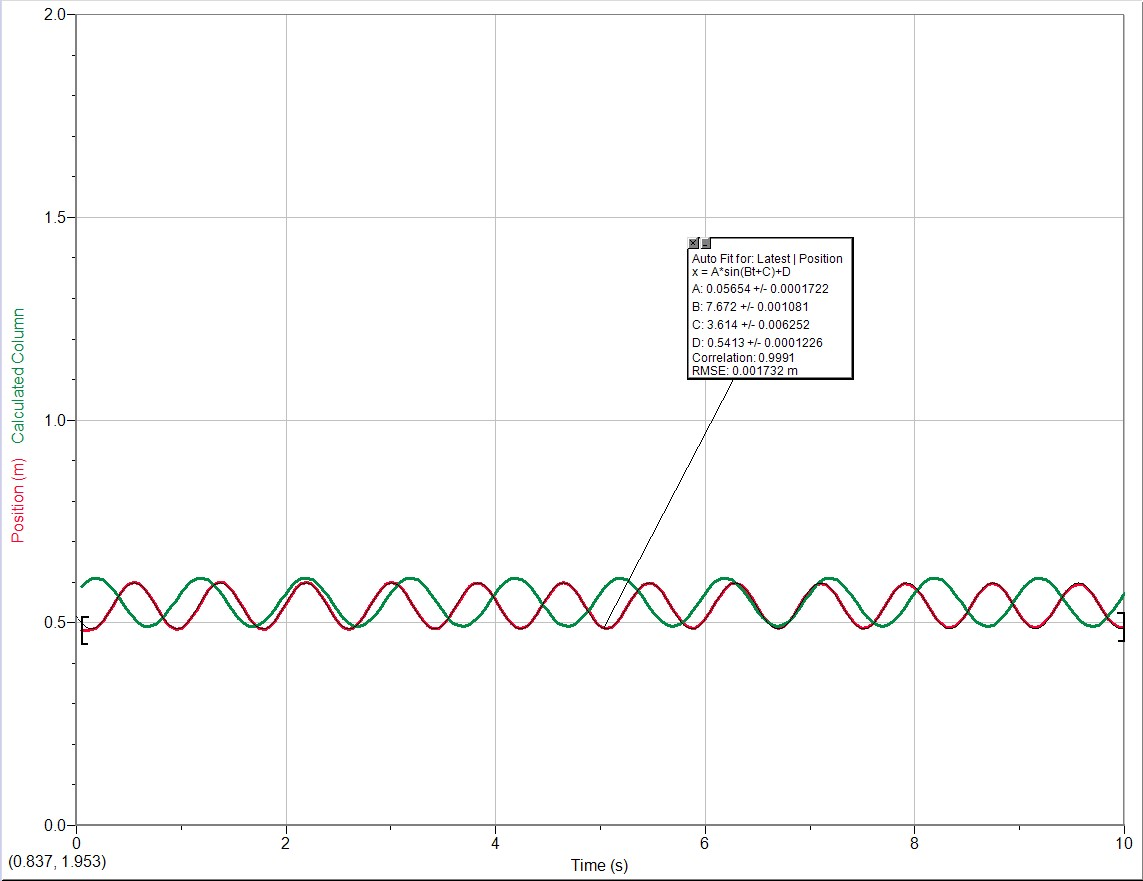
\includegraphics[width=0.8\textwidth]{hangerMassOnly_SHM.jpg}
        \caption{Harmonic Motion of Hanging Mass}
        \label{Sonic Plot}
    \end{subfigure}
    \begin{subfigure}
        \centering
        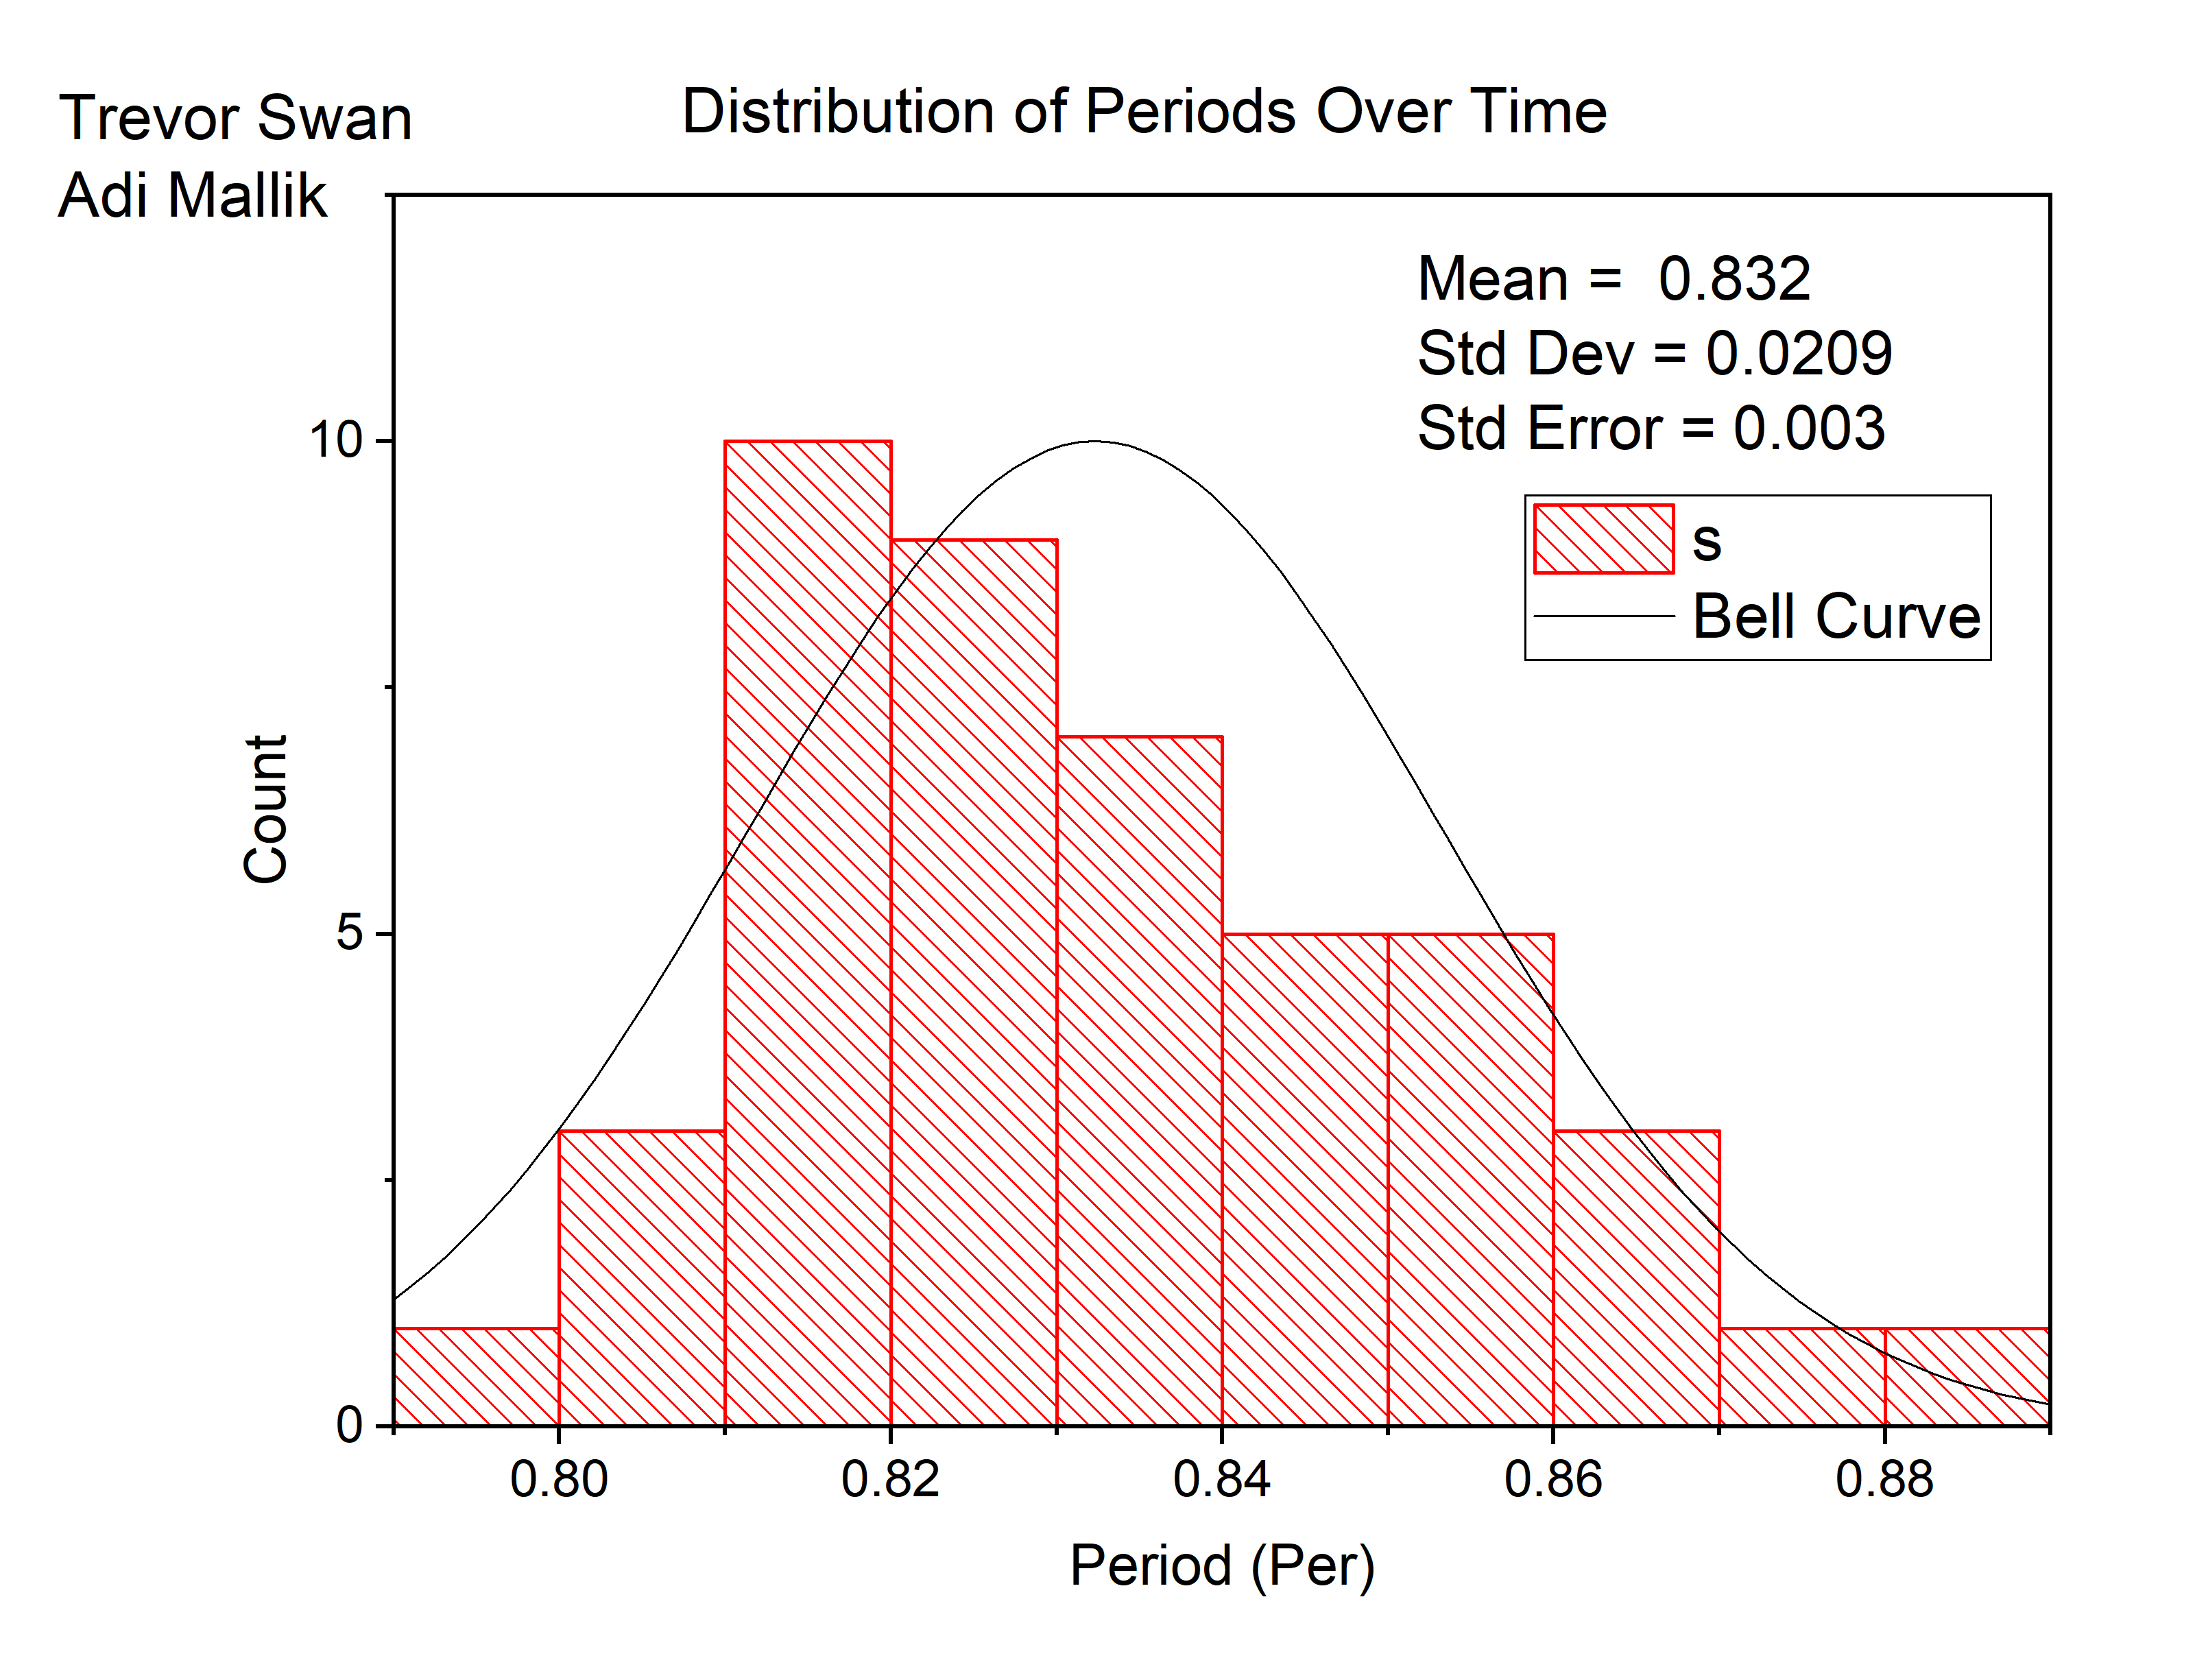
\includegraphics[width=0.8\textwidth]{expT_PEND.jpg}
        \caption{Pendulum Distribution}
        \label{Pend Plot}
    \end{subfigure} 
\end{figure}

% Torsion Modulus Table
\begin{figure}
    \centering
    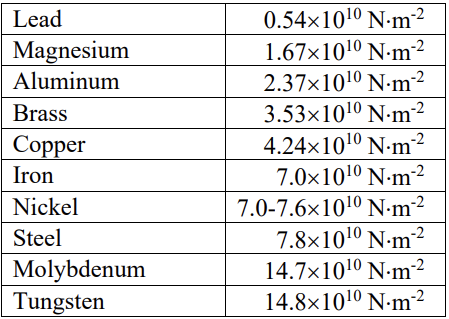
\includegraphics{Torsion_Modulus.png}
    \caption{Torsion Moduli}
    \label{Torsion Moduli}
\end{figure}

% SHM Data
\begin{table}[H]
    \centering
    \begin{tabular}{c c c c c}
        \textbf{Trial} & $x_m$ & $\omega$ & $\phi$ & $x_0$ \\
        \hline \hline % Horizontal line for styling
        \text{Hanger 1} & $0.05654\pm0.000172$ & $7.672\pm0.001081$ & $3.614\pm0.006252$ & $0.5413\pm0.0001226$ \\
        \hline
        \text{Hanger 2} & $0.06036\pm0.0004562$ & $7.681\pm0.003385$ & $0.3487\pm0.02188$ & $0.5280\pm0.0003250$ \\
        \hline
        \text{Hanger 3} & $0.06553\pm0.0001749$ & $7.670\pm0.0009447$ & $1.065\pm0.005451$ & $0.5490\pm0.0001245$ \\
        \hline
        \text{Hanger 4} & $0.6596\pm0.0004576$ & $7.670\pm0.002452$ & $1.105\pm0.01415$ & $0.5445\pm0.0001627$ \\
        \hline
        \text{Large Amp} & $0.1066\pm0.0004402$ & $7.672\pm0.001407$ & $5.861\pm0.008181$ & $0.5481\pm0.0003101$ \\
        \hline
        \text{Large Mass} & $0.2193\pm0.0007210$ & $5.815\pm0.001119$ & $4.824\pm0.006505$ & $0.4264\pm0.0005079$ \\
    \end{tabular}
    \caption{Translational Motion Trials}
    \textit{Not rounded for calculation accuracy}
    \label{Sonic Motion Trials}
\end{table}

\end{document}